\documentclass[../notes.tex]{subfiles}

\pagestyle{main}
\renewcommand{\chaptermark}[1]{\markboth{\chaptername\ \thechapter\ (#1)}{}}
\stepcounter{chapter}

\begin{document}




\chapter{Cycloadditions and Photochemistry}
\section{Problems 2 and 5}
\begin{itemize}
    \item \marginnote{9/6:}We begin with Problem 5.
    \begin{figure}[h!]
        \centering
        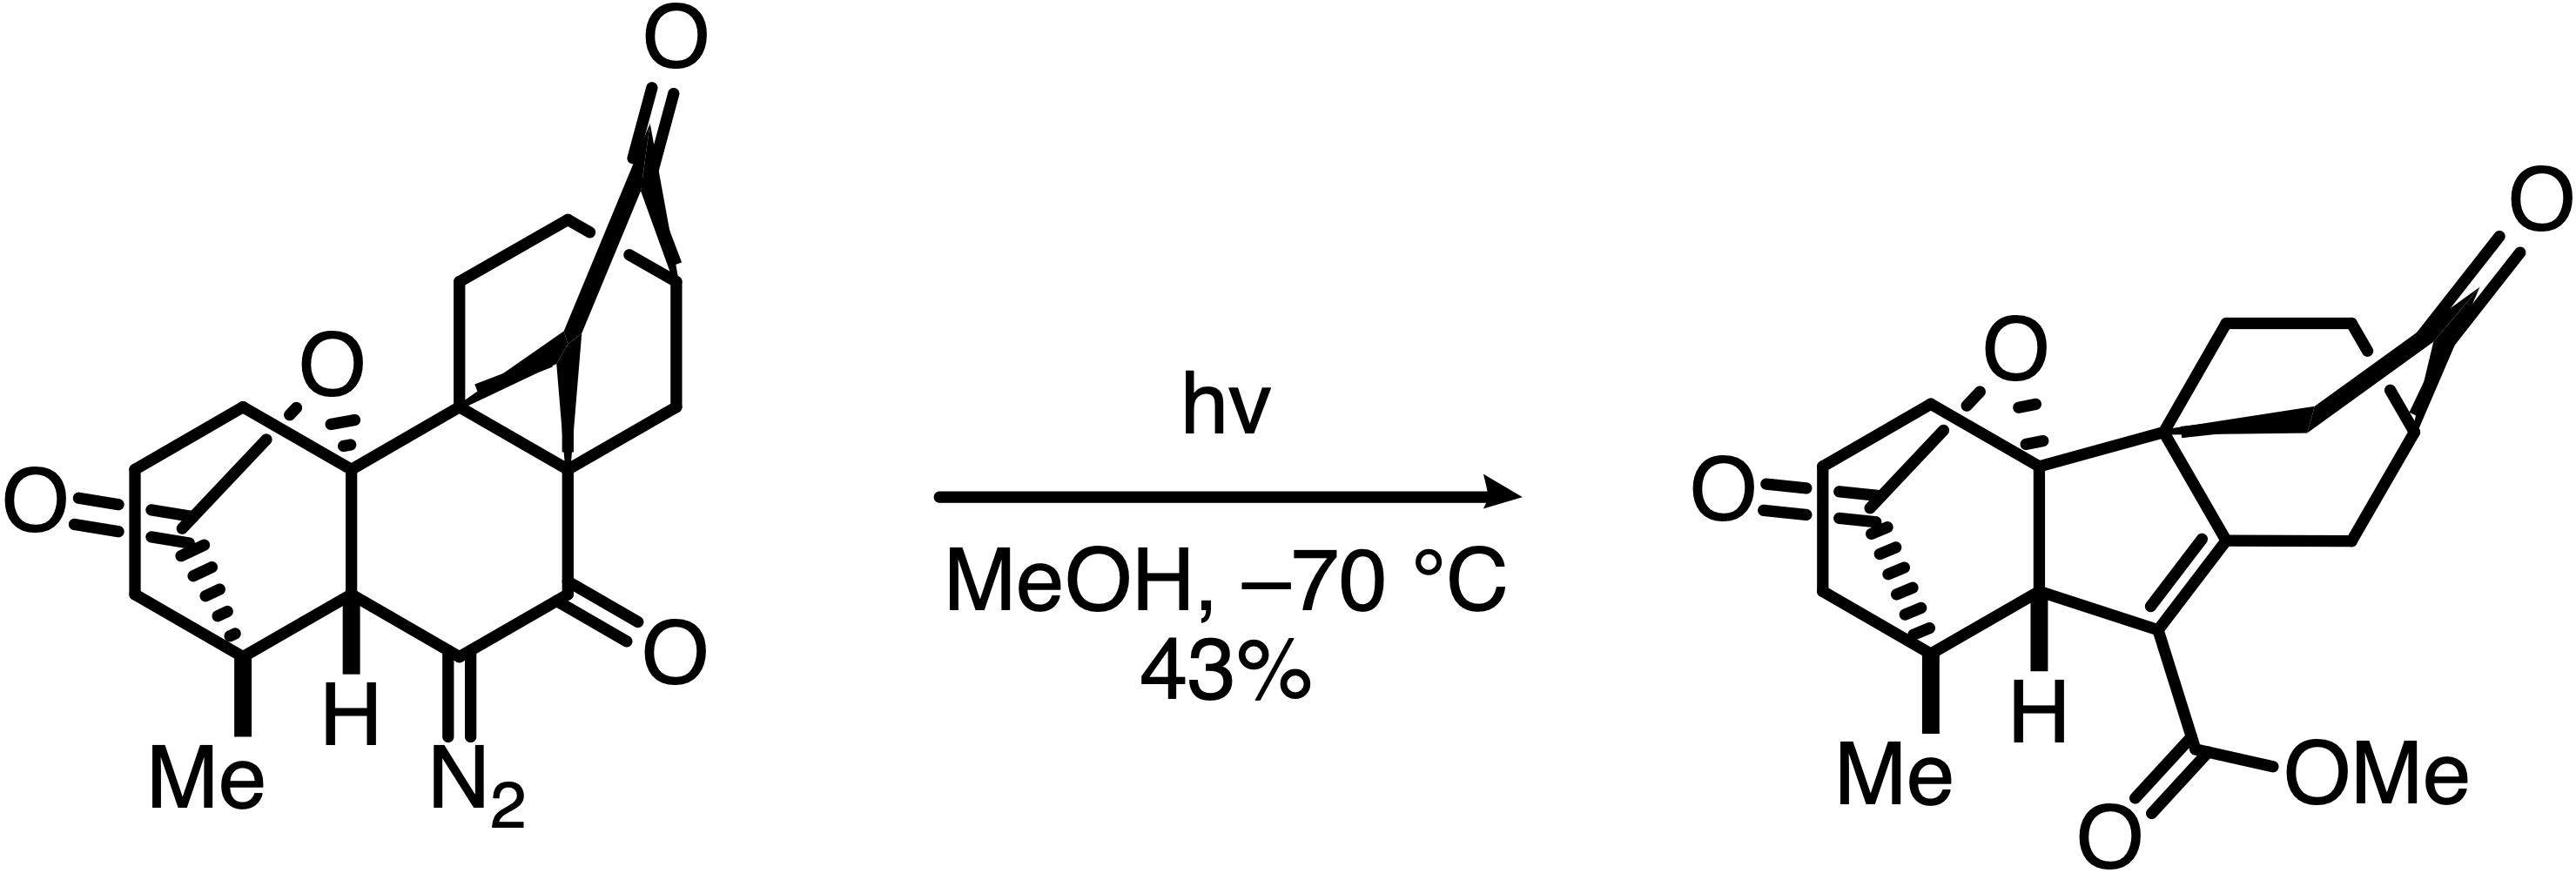
\includegraphics[width=0.5\linewidth]{PSet2Q5.png}
        \caption{PSet 2, Q5.}
        \label{fig:PSet2Q5}
    \end{figure}
    \item The first step --- and the light-activated step --- is a photolytic \textbf{Wolff rearrangement}.
    \begin{itemize}
        \item Specifically, the light will photoexcite the diazo functional group. We don't really need to show this, though.
    \end{itemize}
    \item After that, we have methanol addition to the ketene.
    \begin{itemize}
        \item By using two methanol molecules, we can access a six-membered transition state.
        \item On ketenes.
        \begin{itemize}
            \item The \ce{C=O} and \ce{C=C} $\pi$-bonding orbitals are orthogonal.
            \item More specifically, this means that the \ce{C=O} $\pi$-bond orbital lies in the plane of the page, and the \ce{C=C} $\pi$-bond orbital lies out of the plane of the page.
        \end{itemize}
        \item Implication: We must be careful about choosing the side of the ketene to which the methanol adds.
    \end{itemize}
    \item Hydrogen bonding from methanol stabilizes many of the steps, as drawn in the third intermediate.
    \item There may be a \textbf{retro-Michael addition} somewhere in here. However, this was said to form an enolate, and thus be a step we'd like to avoid??
    \item Jasmin: Where can we learn about photoexcitation problems?
    \begin{itemize}
        \item There are two types of photoexcitation regimes: Broad spectrum and specific wavelength.
        \item The majority of productive photochemical processes use lower energy photons.
        \begin{itemize}
            \item As a consequence, photochemistry is rare among unsaturated systems because anything powerful enough to drive something there will rupture bonds everywhere.
        \end{itemize}
        \item By contrast, conjugated systems are more easily photoexcited.
        \item Example: The most reliable way to generate 4-membered rings is with photoexcitation! We can form 4-membered rings in such a system because we're pumping more than enough energy to overcome the ring strain. Here's how it works.
        \begin{figure}[h!]
            \centering
            \footnotesize
            \schemestart
                \chemfig{-[:30](=[2]O)-[:-30]=_[6]}
                \arrow{->[$h\nu$]}
                \chemleft[
                    \subscheme{
                        \chemfig{-[:30](-[2]\charge{30=\.}{O})=_[:-30]-[6]\charge{0=\.}{}}
                        \arrow{<->}
                        \chemfig{-[:30](=[2]O)-[:-30]\charge{0=\.}{}-[6]\charge{0=\.}{}-[,0.3,,,opacity=0]}
                    }
                \chemright]
                \arrow{->[\chemfig[atom sep=1em]{*6(-----=)}]}
                \chemfig{-[:30](=[2]O)-[:-30]\charge{30=\.}{}-[6]-*6([:30]-----\charge{150=\.}{}-)}
                \arrow
                \chemfig{-[:30](=[2]O)-[:-30]*4([:-45]--*6(-----)--)}
            \schemestop
            \caption{Forming 4-membered rings via photochemistry.}
            \label{fig:4photo}
        \end{figure}
        \begin{itemize}
            \item A $\beta$-unsaturated carbonyl can be excited to a diradical, which can also be thought of as an exited state of the $\pi$-bond.
            \begin{itemize}
                \item Note that the unconjugated alkene does \emph{not} get photoexcited!
            \end{itemize}
            \item Then we can do radical chemistry with the ketone, which is hard to excite.
        \end{itemize}
        \item You could also have photoexcitation followed by intersystem crossing (singlet to triplet state).
        \item We will likely learn more about photoexcitation in 5.53.
        \item Takeaway: Looking at the starting material, we should identify conjugated systems, like how the ketone is conjugated to the $\beta$-\ce{C=N} bond.
    \end{itemize}
    \item Aside: Rhodium can do very similar chemistry under thermal conditions. Instead of a carbene, we'd get a metal alkylidene, but it'd be the same end product.
    \begin{itemize}
        \item So this can be transition-metal catalyzed.
    \end{itemize}
    \item Reference: \textcite{bib:PSet2Q5}.
    \item Altogether, the full solution to PSet 2, Q5 is on the next page.
    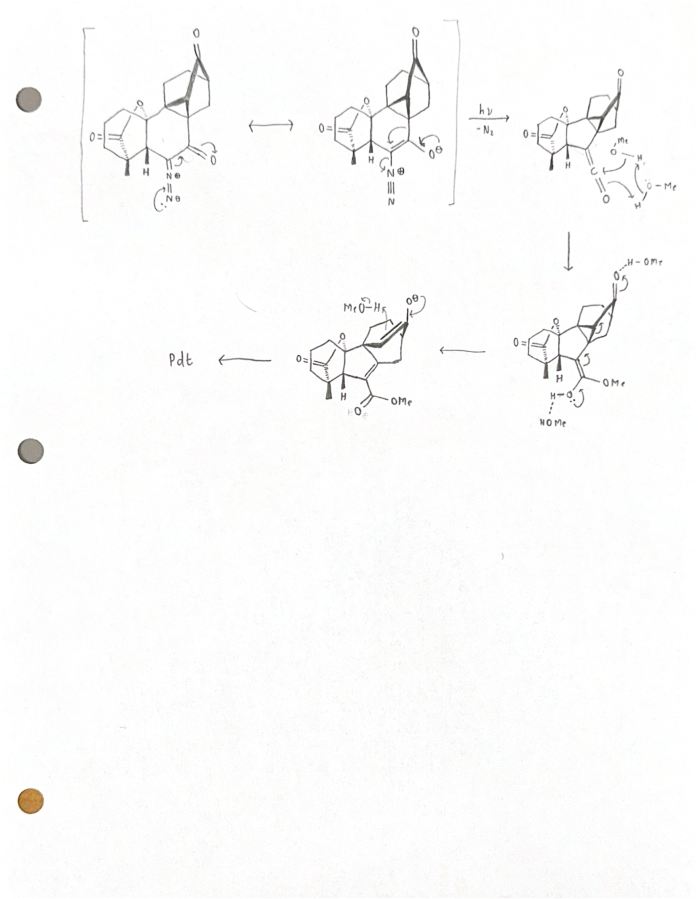
\includepdf{ExtFiles/PSet2Q5Full.pdf}
    \item We now begin PSet 2, Q2.
    \begin{figure}[h!]
        \centering
        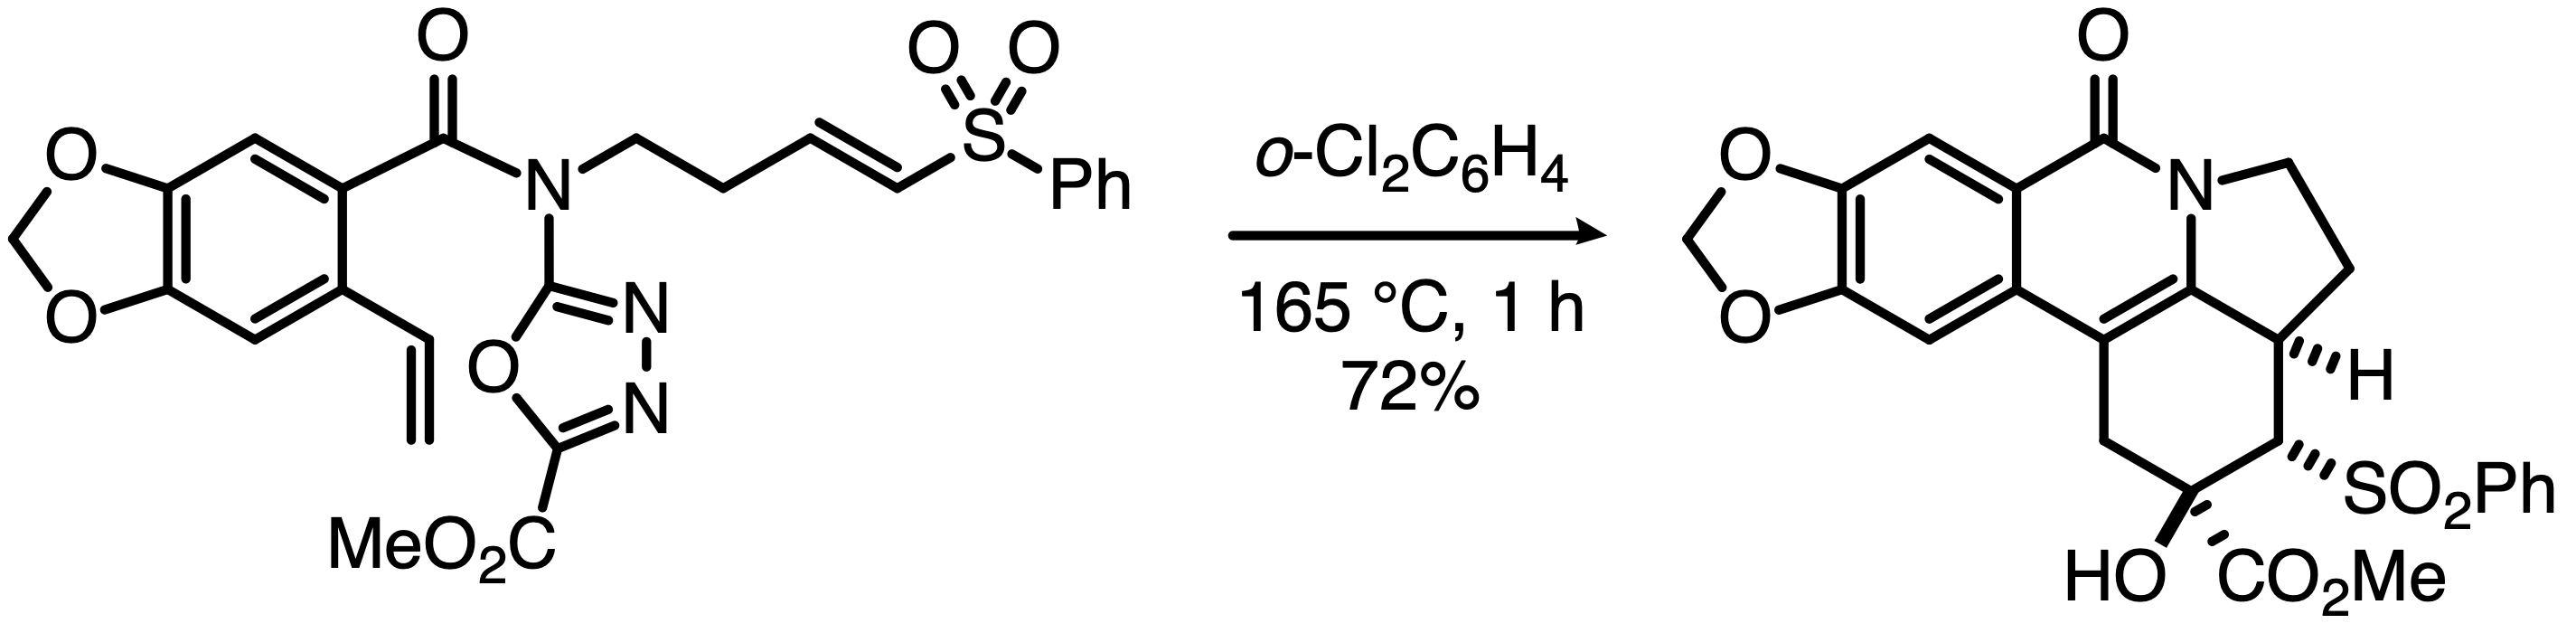
\includegraphics[width=0.65\linewidth]{PSet2Q2.png}
        \caption{PSet 2, Q2.}
        \label{fig:PSet2Q2}
    \end{figure}
    \item Starts off with a $[4+2]$ cycloaddition, which will follow similar rules to the analogous Diels-Alder.
    \begin{itemize}
        \item For example, this cycloaddition will also be diastereoselective, and hence will prefer to have the phenylsulfonyl EWG be \emph{endo} in the transition state.
        \begin{itemize}
            \item This sets the stereochemistry of the right side of the molecule.
        \end{itemize}
        \item This is an antarafacial/suprafacial reaction, not a suprafacial/suprafacial reaction.
        \begin{itemize}
            \item Read up on the \textbf{Woodward-Hoffmann rules}!!
        \end{itemize}
        \item Forming a 5-membered ring is better than a six-membered ring??
        \item Note that we choose to react with the more electron-poor alkene because it has a lower, more energetically accessible LUMO.
    \end{itemize}
    \item After the cycloaddition, we rearrange the electrons and spit out nitrogen.
    \item We then do another $[4+2]$ cycloaddition.
    \begin{itemize}
        \item How do we retain the stereochemistry at the carbanion?? What's the alternate mechanism?
    \end{itemize}
    \item At high temperature, the \ce{N-O} ketal can drop down and (reversibly) expel the oxygen.
    \begin{itemize}
        \item The formation of the \ce{N}-acyl iminium will seriously labilize the $\alpha$-carbon's hydrogens. The labilization effect is so extreme that any base in solution --- from the starting material, to something intramolecular, to the unsilylated glass of the reaction vessel --- will pick it off.
    \end{itemize}
    \item Then we just have to protonate the oxygen and we're done!
    \item Altogether, the full solution to PSet 2, Q2 is on the next page.
    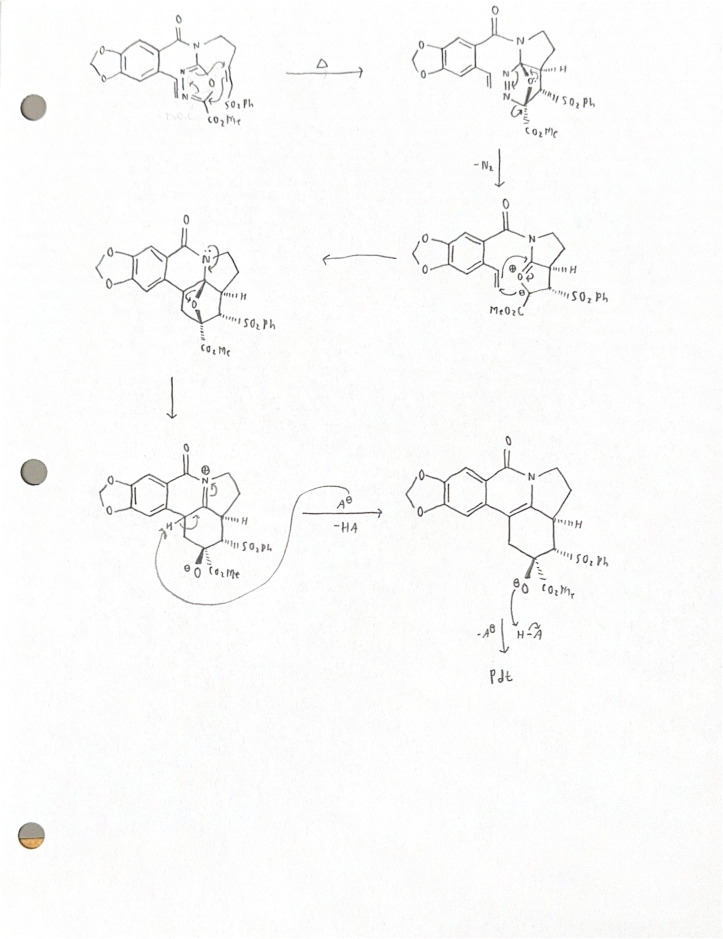
\includepdf{ExtFiles/PSet2Q2Full.pdf}
    \item Definitely have all of PSet 2 ready for next Monday!! And have at least looked at PSet 3.
    \begin{itemize}
        \item PSet 2, Q3 is gonna need really good 3D transition state structures. Make sure to try this one!! Hints:
        \begin{itemize}
            \item You start with a Diels-Alder. Lewis acid activates the ketone.
            \item This lowers the energy of the LUMO; sets the stage for an intramolecular Diels-Alder.
            \item Following this, draw the intermediate, put it in a chair scenario, and then sort out the azide.
            \item Azides and Lewis acids can add into the carbonyl. This will lead to loss of \ce{N2}, and how can we facilitate this?
            \begin{itemize}
                \item Schmidt reaction.
            \end{itemize}
            \item Lots of antiperiplanar interactions that are responsible for product distribution.
            \begin{itemize}
                \item This problem is something of a sequel to PSet 1, Q3.
            \end{itemize}
        \end{itemize}
        \item We will start next time with PSet 2, Q3.
    \end{itemize}
    \item Remember to take more pictures!!
    \item Use whatever time we have for this class to think about future problems, not clean copying notes.
    \item Jasmin and I will start next time with two PSet 2 problems; one of us will take Q3, the other Q1.
    \item Focus on PSet 2, but we can start PSet 3.
\end{itemize}




\end{document}